\section*{Appendix: Distinction Centrality in Hierarchical Trees}
\label{sec:appendix-rooted-trees}

To explore the behavior of distinction centrality within strict hierarchical structures, we compute the metric across several balanced, undirected rooted trees. These structures classically model organizational hierarchies, varying in depth (number of management layers) and branching factor (span of control). 

\begin{figure}[ht!]
    \centering
    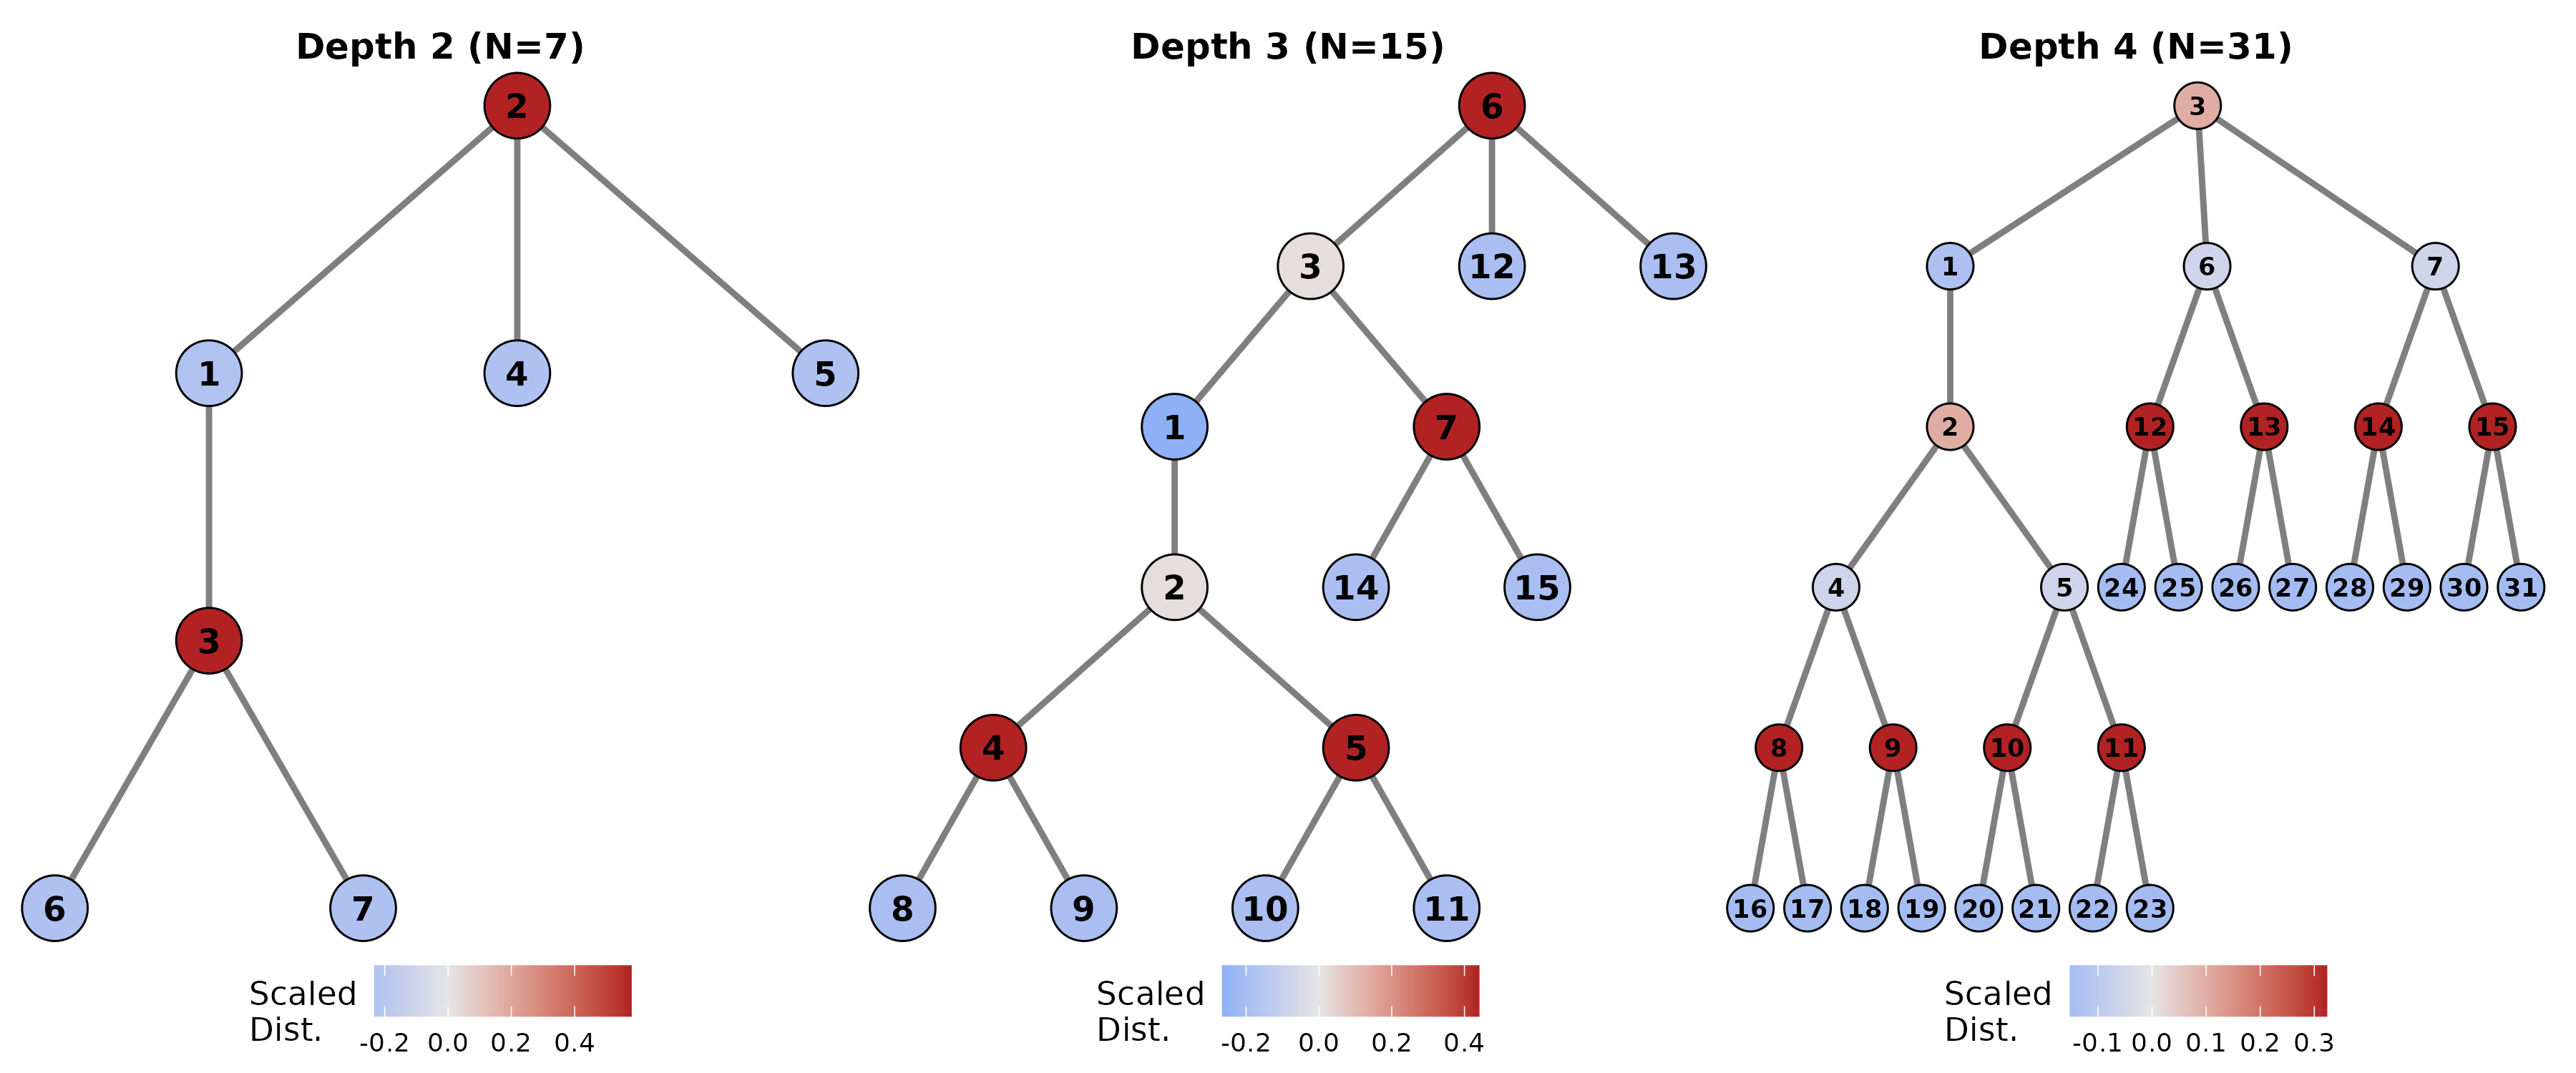
\includegraphics[width=\linewidth]{Plots/tree_comparisons.png}
    \caption{A comparison of distinction centrality ($\beta_i$) across three different hierarchical structures: a binary tree of Depth 2, a binary tree of Depth 3, and a binary tree of Depth 4. Nodes are colored by their scaled distinction scores.}
    \label{fig:tree-comparisons}
\end{figure}

Table \ref{tab:tree-results} displays the computational results for a Depth 2 binary tree (order 7) using the absolute maximum (\texttt{abm}) normalization scheme. The global scalar adjustment factor ($\alpha = \bar{\kappa} / \bar{s}$) for this specific network is approximately $0.7714$.

\begin{table}[ht!]
    \centering
    \begin{tabular}{l l r r r}
    \hline
    \textbf{Node ID} & \textbf{Structural Role} & \textbf{Scaled Distinction ($\beta_i$)} & \textbf{Status ($s_i$)} & \textbf{Constraint ($\kappa_i$)} \\
    \hline
    1 & Root & -0.2286 & 1.0000 & 1.0000 \\
    2, 3 & Middle Branches & 0.5790 & 1.0000 & 0.1925 \\
    4, 5, 6, 7 & Pendant Leaves & -0.2323 & 0.5000 & 0.6180 \\
    \hline
    \end{tabular}
    \caption{Distinction centrality metrics for nodes in the Depth 2 rooted binary tree.}
    \label{tab:tree-results}
\end{table}

\subsection*{The Leverage of Middle Management}
Perhaps counter-intuitively, the highest distinction scores in a strict Depth-2 hierarchy are not held by the root node, but rather by the middle branches (Nodes 2 and 3). While the middle branches share the maximum status ($s_i = 1.0$) with the root node, they experience substantially less constraint ($\kappa_i = 0.1925$). If a middle branch node is deleted, its pendant leaves become structurally isolated components, dropping their status to zero, while the root node loses half of its influence. Therefore, middle managers possess immense structural leverage: their structural ``exit'' destroys the status of their dependents rather than empowering them. 

\subsection*{The Effect of Hierarchical Depth}
As shown in Figure \ref{fig:tree-comparisons}, increasing the depth of the hierarchy shifts who holds the structural leverage. In a deep hierarchy (e.g., Depth 3 or Depth 4), distinction is strictly reserved for the layer of management \textit{immediately above the absolute bottom}. 

When we add a third or fourth layer, the constraint on the top-level senior managers skyrockets. This occurs because deleting a high-level manager no longer isolates their subordinates. Instead, the remaining subordinates form cohesive sub-components. Because the deleted component retains strong local structure, it retains high status, meaning the high-level manager is heavily constrained by the fact that their subordinates can function cohesively without them.

\subsection*{The Span of Control (Branching Factor)}
Distinction is also highly sensitive to the span of control. If we hold depth constant but increase the number of subordinates per manager from 2 (Binary) to 3 (Ternary), the distinction score of the middle managers increases, as does the overall scalar ($\alpha$) of the network. A wider span of control means there are vastly more leaves at the bottom of the hierarchy that have low structural distinction and high constraint. This drags down the average status ($\bar{s}$) of the entire network, mathematically inflating $\alpha$. Middle managers effectively extract more distinction because they monopolize bridging pathways over a larger, more heavily constrained base of subordinates.

\subsection*{The Special Case of the Pure Autocrat (Star Graph Exception)}
We can derive a simplified, exact mathematical expression for the scaled distinction of the root node in any balanced hierarchical tree of Depth $\ge 2$. Because the root is maximally central, its status is one ($s_{root} = 1$). Removing the root shatters the graph into identical sub-trees whose new roots achieve maximum status, rendering the average constraint $\kappa_{root} = 1$. This yields a fixed distinction for the root of:
\begin{equation}
    \beta_{root} = \alpha(1) - 1 = \alpha - 1
\end{equation}
Because the global scalar $\alpha$ is almost always less than 1, the root node of a strict hierarchy will \textit{always} possess negative distinction. Their dominance is highly precarious: deleting the root immediately catapults their direct subordinates to maximum structural status.

However, \textbf{this rule only applies if the tree has middle management (Depth $\ge 2$)}. If the hierarchy is perfectly flat—a pure Star Graph (Depth 1)—the constraint of the root drops to exactly zero. Deleting the root of a star graph isolates every single alter, dropping their eigenvector status to 0. Thus, the root of a star graph achieves maximum positive distinction ($\beta_{root} = \alpha(1) - 0 = \alpha$). 

This elegantly formalizes the classic dilemma of bureaucratic control: the only way to be a truly unconstrained autocrat is to maintain a flat organization where everyone reports directly to the center. But as scale forces the addition of middle management, the center becomes structurally constrained ($\beta_{root} = \alpha - 1$), and structural leverage immediately transfers to the managers directly controlling the lowest levels.